\documentclass[12pt, a4paper]{report}
\usepackage[utf8]{inputenc}
\usepackage[english, russian]{babel}

\usepackage{graphicx}
\usepackage{listings}
\usepackage{color}

\usepackage{amsmath}
\usepackage{pgfplots}
\usepackage{url}
\usepackage{flowchart}
\usepackage{tikz}
\DeclareGraphicsExtensions{.pdf,.png,.jpg,.svg}
\usetikzlibrary{shapes, arrows}

\usepackage{pgfplotstable}

\renewcommand\contentsname{Содержание}

\usepackage{geometry}
\geometry{left=3cm}
\geometry{right=1cm}
\geometry{top=2cm}
\geometry{bottom=2cm}

\lstset{ %
language=C++,                 % выбор языка для подсветки (здесь это С)
basicstyle=\small\sffamily, % размер и начертание шрифта для подсветки кода
numbers=left,               % где поставить нумерацию строк (слева\справа)
numberstyle=\tiny,           % размер шрифта для номеров строк
stepnumber=1,                   % размер шага между двумя номерами строк
numbersep=-5pt,                % как далеко отстоят номера строк от         подсвечиваемого кода
backgroundcolor=\color{white}, % цвет фона подсветки - используем         \usepackage{color}
showspaces=false,            % показывать или нет пробелы специальными     отступами
showstringspaces=false,      % показывать или нет пробелы в строках
showtabs=false,             % показывать или нет табуляцию в строках
frame=single,              % рисовать рамку вокруг кода
tabsize=2,                 % размер табуляции по умолчанию равен 2 пробелам
captionpos=t,              % позиция заголовка вверху [t] или внизу [b] 
breaklines=true,           % автоматически переносить строки (да\нет)
breakatwhitespace=false, % переносить строки только если есть пробел
escapeinside={\%*}{*)},   % если нужно добавить комментарии в коде
keywordstyle=\color{blue}\ttfamily,
stringstyle=\color{red}\ttfamily,
commentstyle=\color{green}\ttfamily,
morecomment=[l][\color{magenta}]{\#},
columns=fullflexible }

\usepackage{titlesec}
\titleformat{\chapter}[hang]{\LARGE\bfseries}{\thechapter{.} }{0pt}{\LARGE\bfseries}
\titleformat*{\section}{\Large\bfseries}
\titleformat*{\subsection}{\large\bfseries}

\begin{document}

    \begin{titlepage}

        \begin{center}
            \Large
            {\sl Государственное образовательное учреждение высшего профессионального образования\\
            {\bf«Московский государственный технический университет имени Н.Э. Баумана»\\
				(МГТУ им. Н.Э. Баумана)}}
				\noindent\rule{\textwidth}{2pt}
            \vspace{3cm}

			{\scshape\LARGE Рубежный контроль №2 \par}
			\vspace{0.5cm}	
			{\scshape\LARGE по курсу «Анализ алгоритмов» \par}
			\vspace{1.5cm}
			{\huge\bfseries Конечные автоматы и регулярные выражения \par}
			\vspace{2cm}
			\Large Выполнил: Сорокин А.П., гр. ИУ7-52Б\\
			\vspace{0.5cm}
			{\Large Преподаватели: Волкова Л.Л., Строганов Ю.В.}
		
			\vfill
			\Large \textit {Москва, 2019 г.}
            
        \end{center}

    \end{titlepage}
	
	\tableofcontents

	\chapter*{Введение}
	\addcontentsline{toc}{chapter}{Введение}
	Цель лабораторной работы: при помощи конечного автомата и регулярного выражения
	написать программу для поиска критических секций в коде.

    \chapter{Аналитическая часть}
	В данном разделе будут описаны конечные автоматы и регулярные выражения.
	
	\section{Конечные автоматы}
	Конечные автоматы - это упрощенная модель компьютера, имеющая конечное
	число состояний, которая жертвует всеми особенностями компьютеров такие как ОЗУ,
	постоянная память, устройства ввода-вывода и процессорными ядрами в обмен на простоту
	понимания, удобство рассуждения и легкость программной или аппаратной реализации ~\cite{ka}.
	С помощью конечных автоматов можно реализовать такие вещи как, регулярные выражения, лексический анализатор, ИИ в играх и тд.

	\section{Регулярные выражения}
	Регулярные выражения — язык поиска подстроки или подстрок в тексте. Для поиска
	используется паттерн (шаблон, маска), состоящий из символов и метасимволов (символы,
	которые обозначают не сами себя, а набор символов).
	
	Это довольно мощный инструмент, который может пригодиться во многих случая —
	поиск, проверка на корректность строки и т.д. Спектр его возможностей трудно уместить
	в одну статью ~\cite{exp}.
	
	\chapter{Конструкторская часть}
	В данном разделе будет построены конечный автомат и регулярное выражение для решения поставленной задачи.

	\begin{figure}[ht!]
		\centering
		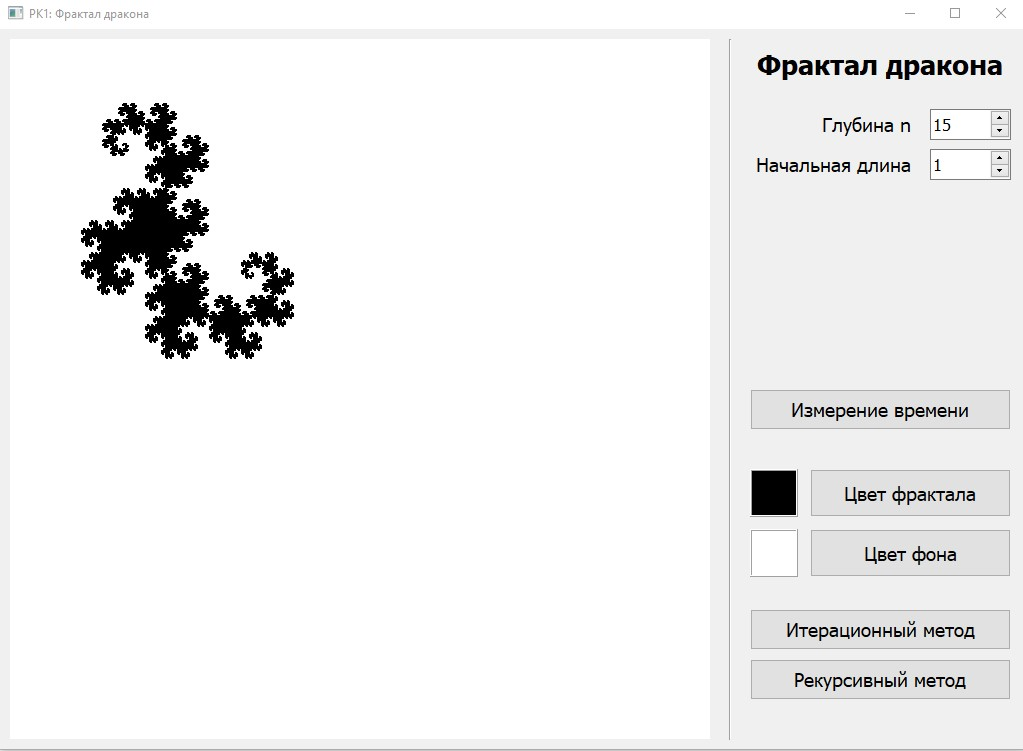
\includegraphics[width=0.8\linewidth]{example_1.jpg}
		\caption{Конечный автомат}
		\label{ris:ka}
	\end{figure}

	\begin{figure}[ht!]
		\centering
		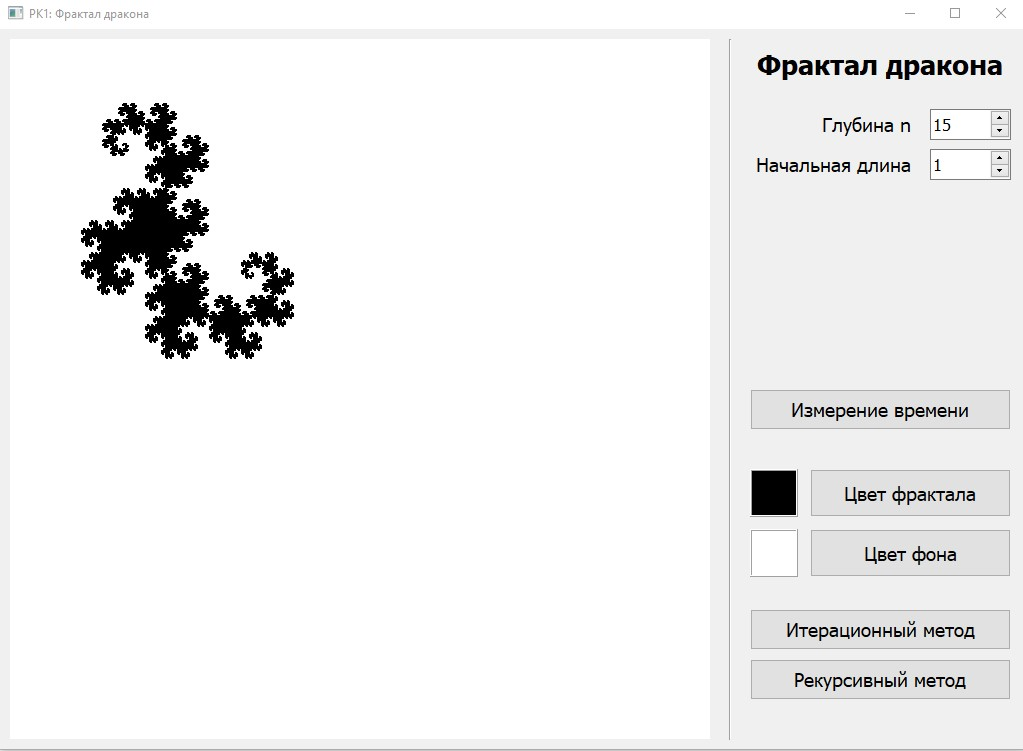
\includegraphics[width=0.8\linewidth]{example_1.jpg}
		\caption{Регулярное выражение}
		\label{risLregexp}
	\end{figure}

	\chapter{Технологическая часть}
	\section{Средства реализации}
	Для реализации программы был использован язык Python ~\cite{Python} (версия интерпретатора 3.7). Для измерения времени была взята функция time.time() из
	библиотеки time. Данный язык обусловлен тем, что функции необходимые для реализации регулярного
	выражения находятся в встроенной библиотеке re.
	
	\section{Реализации алгоритмов}
	На листингах 3.1 - 3.2 представлены коды реализации алгоритмов построения фрактала.
	\begin{lstlisting}[label=some-code,caption=Итерационная реализация]
	std::vector<Point> get_dragon_fractal(Point p1, Point p2, int n)
	{
		std::vector<Point> line;
		line.push_back(p1);
		line.push_back(p2);
	
		for (int i = 0; i < n; i++)
		{
			int xc = line.back().x(), yc = line.back().y();
			int old_size = line.size();
			for (int j = old_size - 2; j >= 0; j--)
			{
				int xx = xc + (line[j].y() - yc);
				int yy = yc - (line[j].x() - xc);
				line.push_back(Point(xx, yy));
			}
		}
	
		return line;
	}
	\end{lstlisting}

	\begin{lstlisting}[label=some-code,caption=Рекурсивная реализация]
	std::vector<Point> get_dragon_fractal_rec(std::vector<Point> line, int n)
	{
		if (n == 0)
			return line;
	
		std::vector<Point> new_line = get_dragon_fractal_rec(line, n - 1);
	
		int xc = new_line.back().x(), yc = new_line.back().y();
		int old_size = new_line.size();
		for (int j = old_size - 2; j >= 0; j--)
		{
			int xx = xc + (new_line[j].y() - yc);
			int yy = yc - (new_line[j].x() - xc);
			new_line.push_back(Point(xx, yy));
		}
	
		for (auto p : new_line)
			line.push_back(p);
		return line;
	}
	\end{lstlisting}

	\newpage


	\chapter{Экспериментальная часть}
	\section{Примеры работы}
	На рисунках 3.1 и 3.2 представлены примеры работы программы, демонстрирующий правильное выполнение алгоритмов.
	\begin{figure}[ht!]
		\centering
		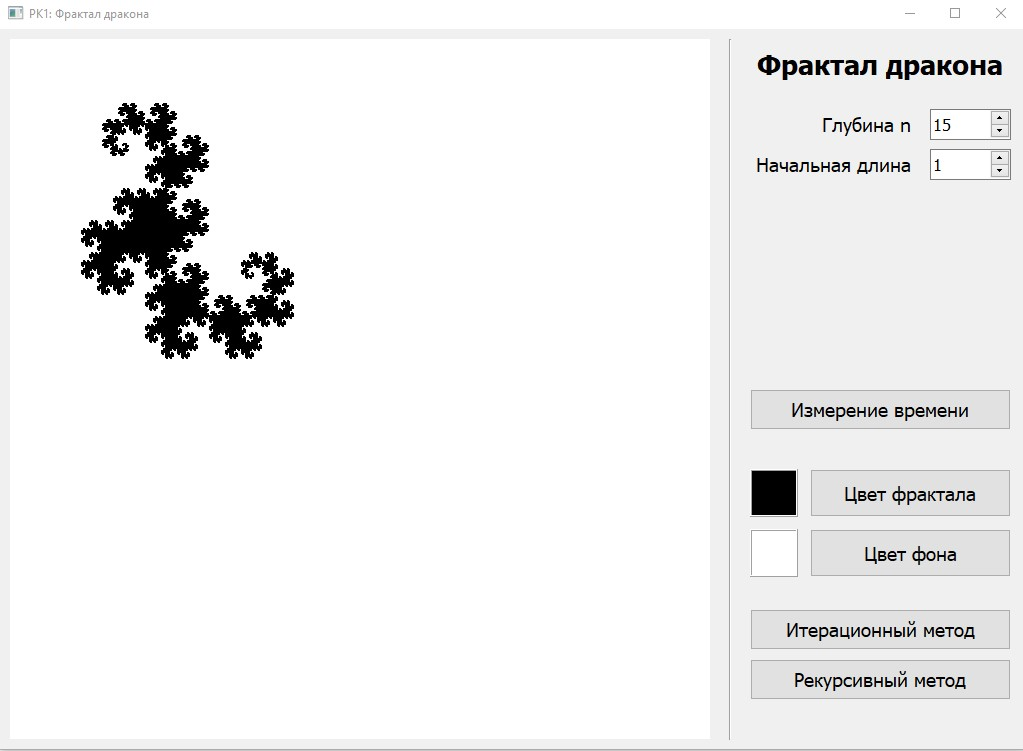
\includegraphics[width=0.8\linewidth]{example_1.jpg}
		\caption{Пример работы программы}
		\label{fig:example}
	\end{figure}
	\begin{figure}[ht!]
		\centering
		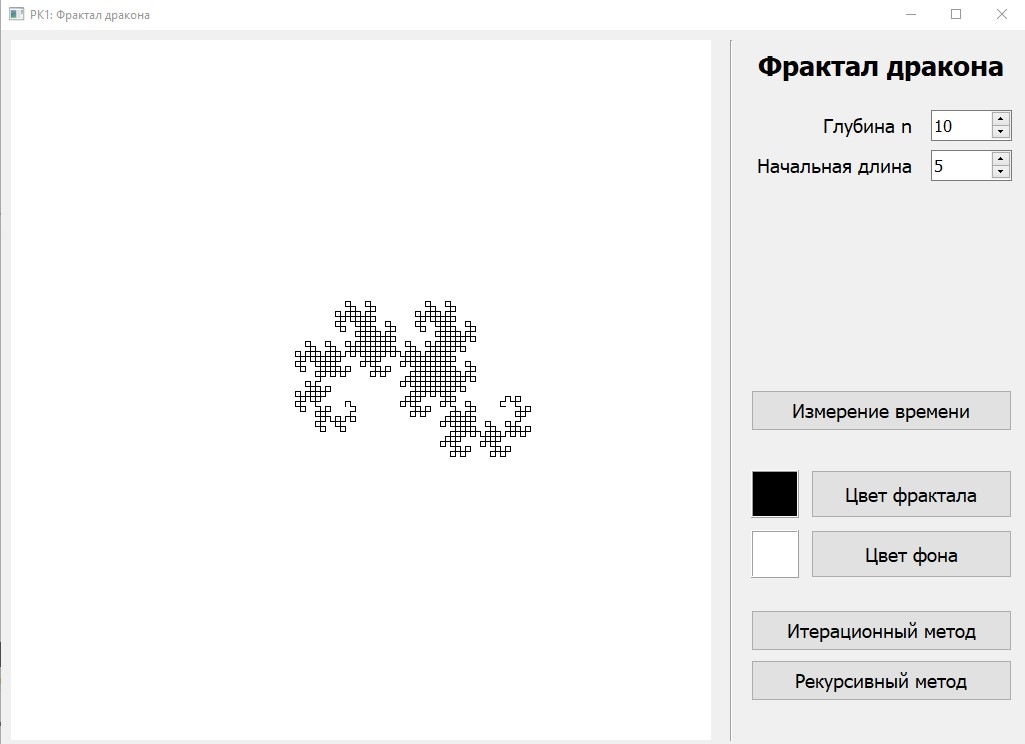
\includegraphics[width=0.8\linewidth]{example_2.jpg}
		\caption{Пример работы программы при увеличенной длины начального отрезка}
		\label{fig:example2}
	\end{figure}
	
	\section{Сравнение работы итерационной и рекурсивной реализации алгоритмов}
	Для сравнения времени работы двух реализаций алгоритмов построения фрактала глубина построения менялась от 1 до 20. Эксперимент для более точного результата повторялся 100 раз. Итоговый результат рассчитывался как средний из полученных результатов. Результаты измерений показаны в таблице 3.1 и на рисунках 3.3, 3.4.\\
	\begin{table}[ht!]
		\caption{Время работы реализаций алгоритмов построения фрактала в тактах процессора}
		\begin{center}
			\pgfplotstabletypeset[
			col sep=semicolon,
			string type,
			columns/Size/.style={column name=Глубина, column type={|c}},
			columns/Iter/.style={column name=Итерационный, column type={|c}},
			columns/Rec/.style={column name=Рекурсивный, column type={|c|}},
			every head row/.style={before row=\hline,after row=\hline},
			every last row/.style={after row=\hline},
			]{time.csv}
		\end{center}
	\end{table}
	
	\begin{figure}[ht!]
		\begin{tikzpicture}
		\begin{axis}
		[%title = График времени работы реализаций алгоритмов построения фрактала,
		table/col sep = semicolon,
		xlabel={Глубина фрактала},
		ylabel={Время в тиках},
		legend pos=outer north east,
		ymajorgrids=true,
		grid style=dashed]
		\addplot[color=red, mark=*] table[x={Size}, y={Iter}] {time.csv};
		\addplot[color=blue, mark=*] table[x={Size}, y={Rec}] {time.csv};
		\legend{Итерационный метод, Рекурсивный метод}
		\end{axis}
		\end{tikzpicture}
		\caption{График времени работы реализаций алгоритмов построения фрактала дракона при глубине}
	\end{figure}

	Можно сделать вывод о том, что рекурсивный алгоритм проигрывает во времени, причём разница во времени стремительно растёт с увеличением глубины.

	\chapter*{Заключение}
	\addcontentsline{toc}{chapter}{Заключение}
	В ходе выполнения рубежного контроля был изучен метод построения фрактала дракона. Для этого были реализованы итерационная и рекурсивная реализация алгоритма построения. Также была оценена эффективность двух реализаций: итерационный метод построения при большой глубине (больше 16) фрактала значительно выигрывает рекурсивный метод.
	
	\newpage
	
	\begin{thebibliography}{}
	\bibitem{ka} Конечные автоматы (finite-state machine) [Электронный ресурс]. - Режим доступа:
	https://habr.com/ru/post/358304/, свободный. (Дата обращения: 5.2.2020 г.)
	\bibitem{regexp} Регулярные выражения [Электронный ресурс]. - Режим доступа:
	https://habr.com/ru/company/badoo/blog/343310/, свободный. (Дата обращения:
	5.2.2020 г.)
	\end{thebibliography}
	\addcontentsline{toc}{chapter}{Литература}

\end{document}
